\usetikzlibrary{arrows.meta}
\begin{frame}[fragile,label=useAfterFree3]{checking use-after-free (3)}
    \lstset{
        language=C,style=script,
        moredelim={**[is][\btHL<2>]{~2~}{~end~}},
    }
\begin{tikzpicture}
\node[anchor=north east] at (-.2, 0) {
\begin{lstlisting}
void someFunction() {
    int *quux = malloc(sizeof(int));
    ...
    // A
    do {
        // B
        ...
        if (anotherFunction()) {
            free(quux);
            // C
        }
        ...
        // D
    } while (complexFunction());
    ...
    // E
    *quux++;
    ...
}
\end{lstlisting}
};
    \tikzset{flow/.style={draw,thick,font=\fontsize{9}{10}\selectfont,anchor=north west},
    flowLine/.style={thick,-Latex},
    flowLineB/.style={very thick,dotted,-Latex},
    }
    \begin{scope}[y=0.8cm]
        \begin{visibleenv}<1->
        \node[flow] (A) at (0, 0) { A: \textit{allocated} };
        \node[flow,alt=<3>{red}{},alt=<1-2>{dashed}] (B) at (1, -1) { B (from \textit{allocated}): \textit{allocated} };
        \draw[flowLine] ([xshift=.5cm]A.south west) |- ([yshift=.1cm]B.west);
        \end{visibleenv}
        \begin{visibleenv}<2->
        \node[flow] (C1) at (1, -2) { C (from \textit{allocated}): quux: \textit{freed} };
            \node[flow,alt=<1-4>{dashed}{}] (D1) at (1, -3) { D (from \textit{freed}): \textit{freed} };
        \node[flow] (E1) at (2, -4) { E (from \textit{freed}): USE-AFTER-FREE };
        \draw[flowLine] ([yshift=-.1cm]B.west) -- ++(-.2cm, 0cm) |- ([yshift=.1cm]C1.west);
        \draw[flowLine] ([yshift=-.1cm]C1.west) -- ++(-.2cm, 0cm) |- ([yshift=.1cm]D1.west);
        \draw[flowLine] ([yshift=-.1cm]D1.west) -- ++(-.2cm, 0cm) |- ([yshift=.1cm]E1.west);
        \end{visibleenv}
        \begin{visibleenv}<3->
        \node[flow,alt=<3>{dashed}{}] (D2) at (1, -5) { D (from \textit{allocated}): \textit{allocated} };
        \draw[flowLine,alt=<3>{red}{}] ([yshift=-.1cm]B.west) -- ++(-.3cm, 0cm) |- ([yshift=.1cm]D2.west);
        \node[flow] (E2) at (2, -6) { E (from \textit{allocated}): ok };
        \draw[flowLine,alt=<3>{red}{}] ([yshift=-.1cm]D2.west) -- ++(-.2cm, 0cm) |- ([yshift=.1cm]E2.west);
        \end{visibleenv} 
        \begin{visibleenv}<4->
        \draw[flowLineB,alt=<4>{red}{}] ([yshift=-.1cm]D2.east) -- ++(2.5cm, 0cm) |- ([yshift=.1cm]B.east);
        \end{visibleenv} 
        \begin{visibleenv}<5->
            \node[flow,alt=<5>{dashed}{}] (B2) at (1, -7) { B (from \textit{freed}): \textit{freed} };
            \draw[flowLine,alt=<5>{red}{}] ([yshift=-.1cm]D1.west) -- ++(-.8cm, 0cm) |- ([yshift=.1cm]B2.west);
            \node[flow] (C2) at (1, -8) { C (from \textit{freed}): DOUBLE-FREE };
            \draw[flowLine] ([yshift=-.1cm]B2.west) -- ++(-.8cm, 0cm) |- ([yshift=.1cm]C2.west);
        \end{visibleenv} 
        \begin{visibleenv}<6->
            \draw[flowLineB,alt=<6>{red}{}] ([yshift=-.1cm]B2.east) -- ++(3cm, 0cm) |- ([yshift=.2cm]D1.east);
        \end{visibleenv}
    \end{scope}
\end{tikzpicture}
\end{frame}

\begin{frame}{result from clang's scan-build}
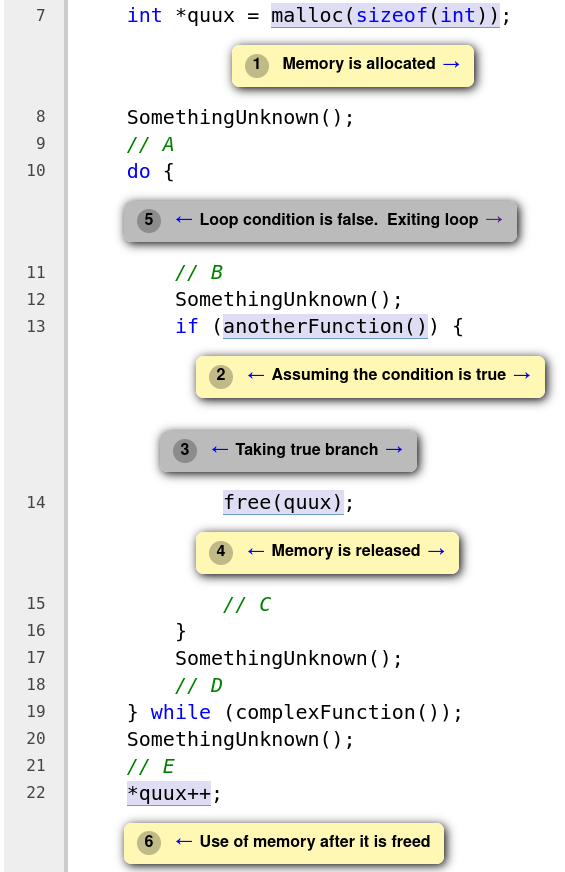
\includegraphics[height=0.9\textheight]{../static/scan-build-uaf-example3a}
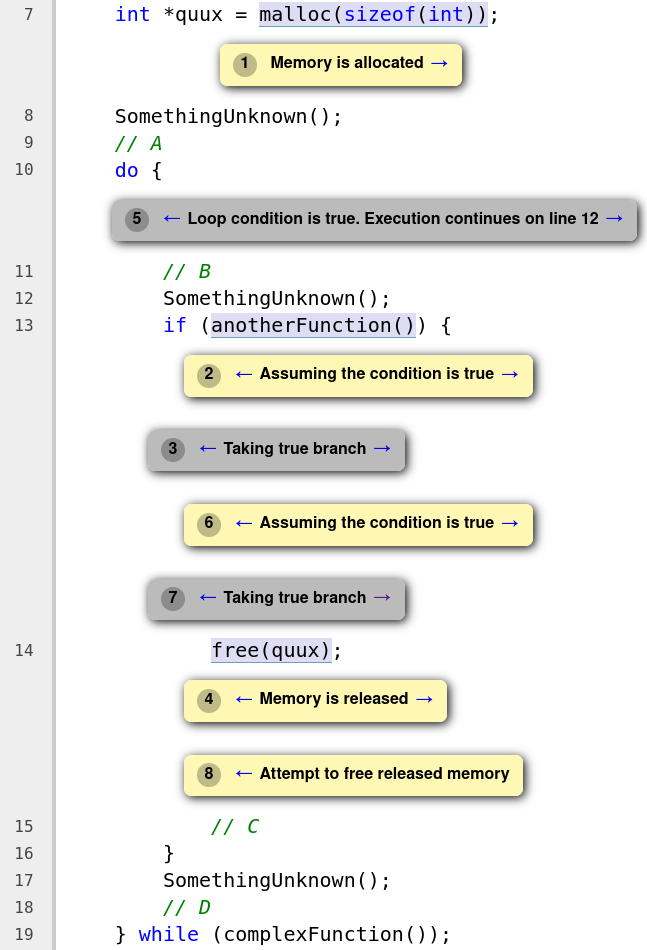
\includegraphics[height=0.9\textheight]{../static/scan-build-uaf-example3b}
\end{frame}
